\section{INTRODUCTION}
\label{sec:introduction}

Every day, billions of people around the world look at RGB screens, and the output displayed on these screens is the output of any software systems. Therefore, the visual representation of interactive digital humans can significantly enhance user experience. The proposed \textbf{DeepGesture} model builds on the DiffuseStyleGesture model \citep{yang2023diffusestylegesture}, leveraging a diffusion model \citep{ho2020denoising} with classifier-free guidance \citep{ho2022classifier} to control features during denoising. Applying diffusion to gesture generation shares similarities with image generation, such as using conditional diffusion on gesture data (analogous to image dimensions) and employing latent vectors in feature encoding/decoding stages. Key differences include conditional generation with emotional states (e.g., emotion vectors and interpolations) and feature fusion via self-attention to relate emotions, seed gestures, and frames (similar to text-image alignment in DALL-E 2), plus concatenating speech and text inputs (analogous to pixel-wise conditions in ControlNet).



%Artificial intelligence (AI) has shown remarkable results in recent years, not only in research but also in practical applications, such as ChatGPT and Midjourney, showcasing vertical and horizontal growth in various fields. Although computer graphics can construct highly realistic human faces, gesture generation has traditionally relied on Motion Capture from sensors, posing significant challenges in building an AI system that learns from data. Generating realistic beat gestures is challenging because gestural beats and verbal stresses are not strictly synchronized, and it is complicated for end-to-end learning models to capture the complex relationship between speech and gestures.

%With the success of large language models in text processing and the advancement of Computer-generated imagery (CGI) in producing nearly indistinguishable human faces, combined with the increasing ease and accuracy of human speech synthesis, gesture generation through AI has become one of the main bottlenecks in developing interactive digital human.

%Therefore, the rendering of each pixel on the screen and the realistic simulation of images have been a focus of computer graphics scientists since the 1960s, particularly in the simulation of human figures or digital human.

%Today, computer graphics technology can realistically simulate many complex objects such as water, roads, bread, and even human bodies and faces with incredible detail, down to individual hair strands, pimples, and eye textures. In 2015, using 3D scanning techniques \citep{metallo2015scanning} to capture all angles of the face and light reflection, researchers were able to recreate President Obama's face on a computer with high precision, making it almost indistinguishable from the real thing.


\subsection{Gesture Generation Problem Statement}
\label{sec:Data}

\begin{figure}[h]
	\centering
	\begin{subfigure}{0.2\linewidth}
		\centering
		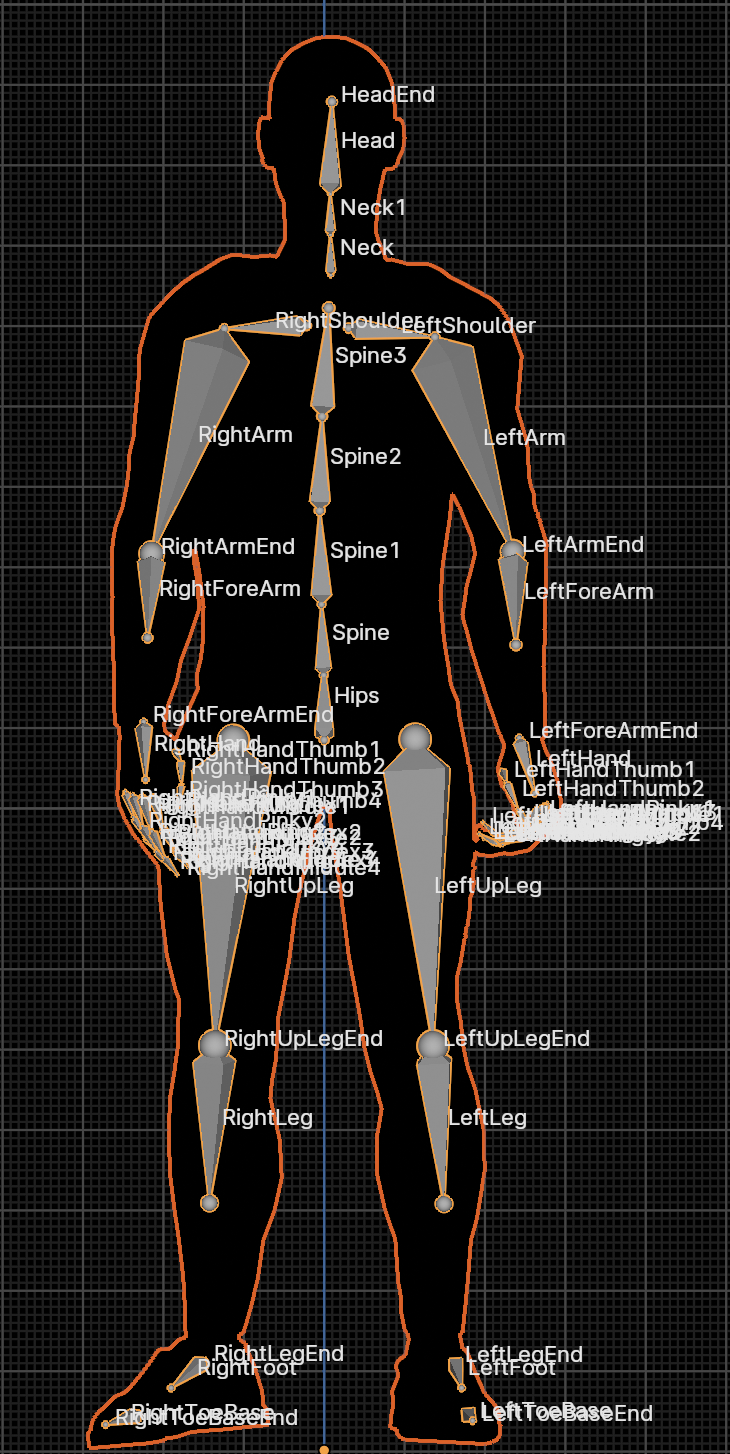
\includegraphics[height=4cm]{figures/Skeleton.png}
		\caption{\small Skeleton and joint names of single frame}
		\label{fig:Skeleton}
	\end{subfigure}
	\hfill
	\begin{subfigure}{0.75\linewidth}
			\centering
			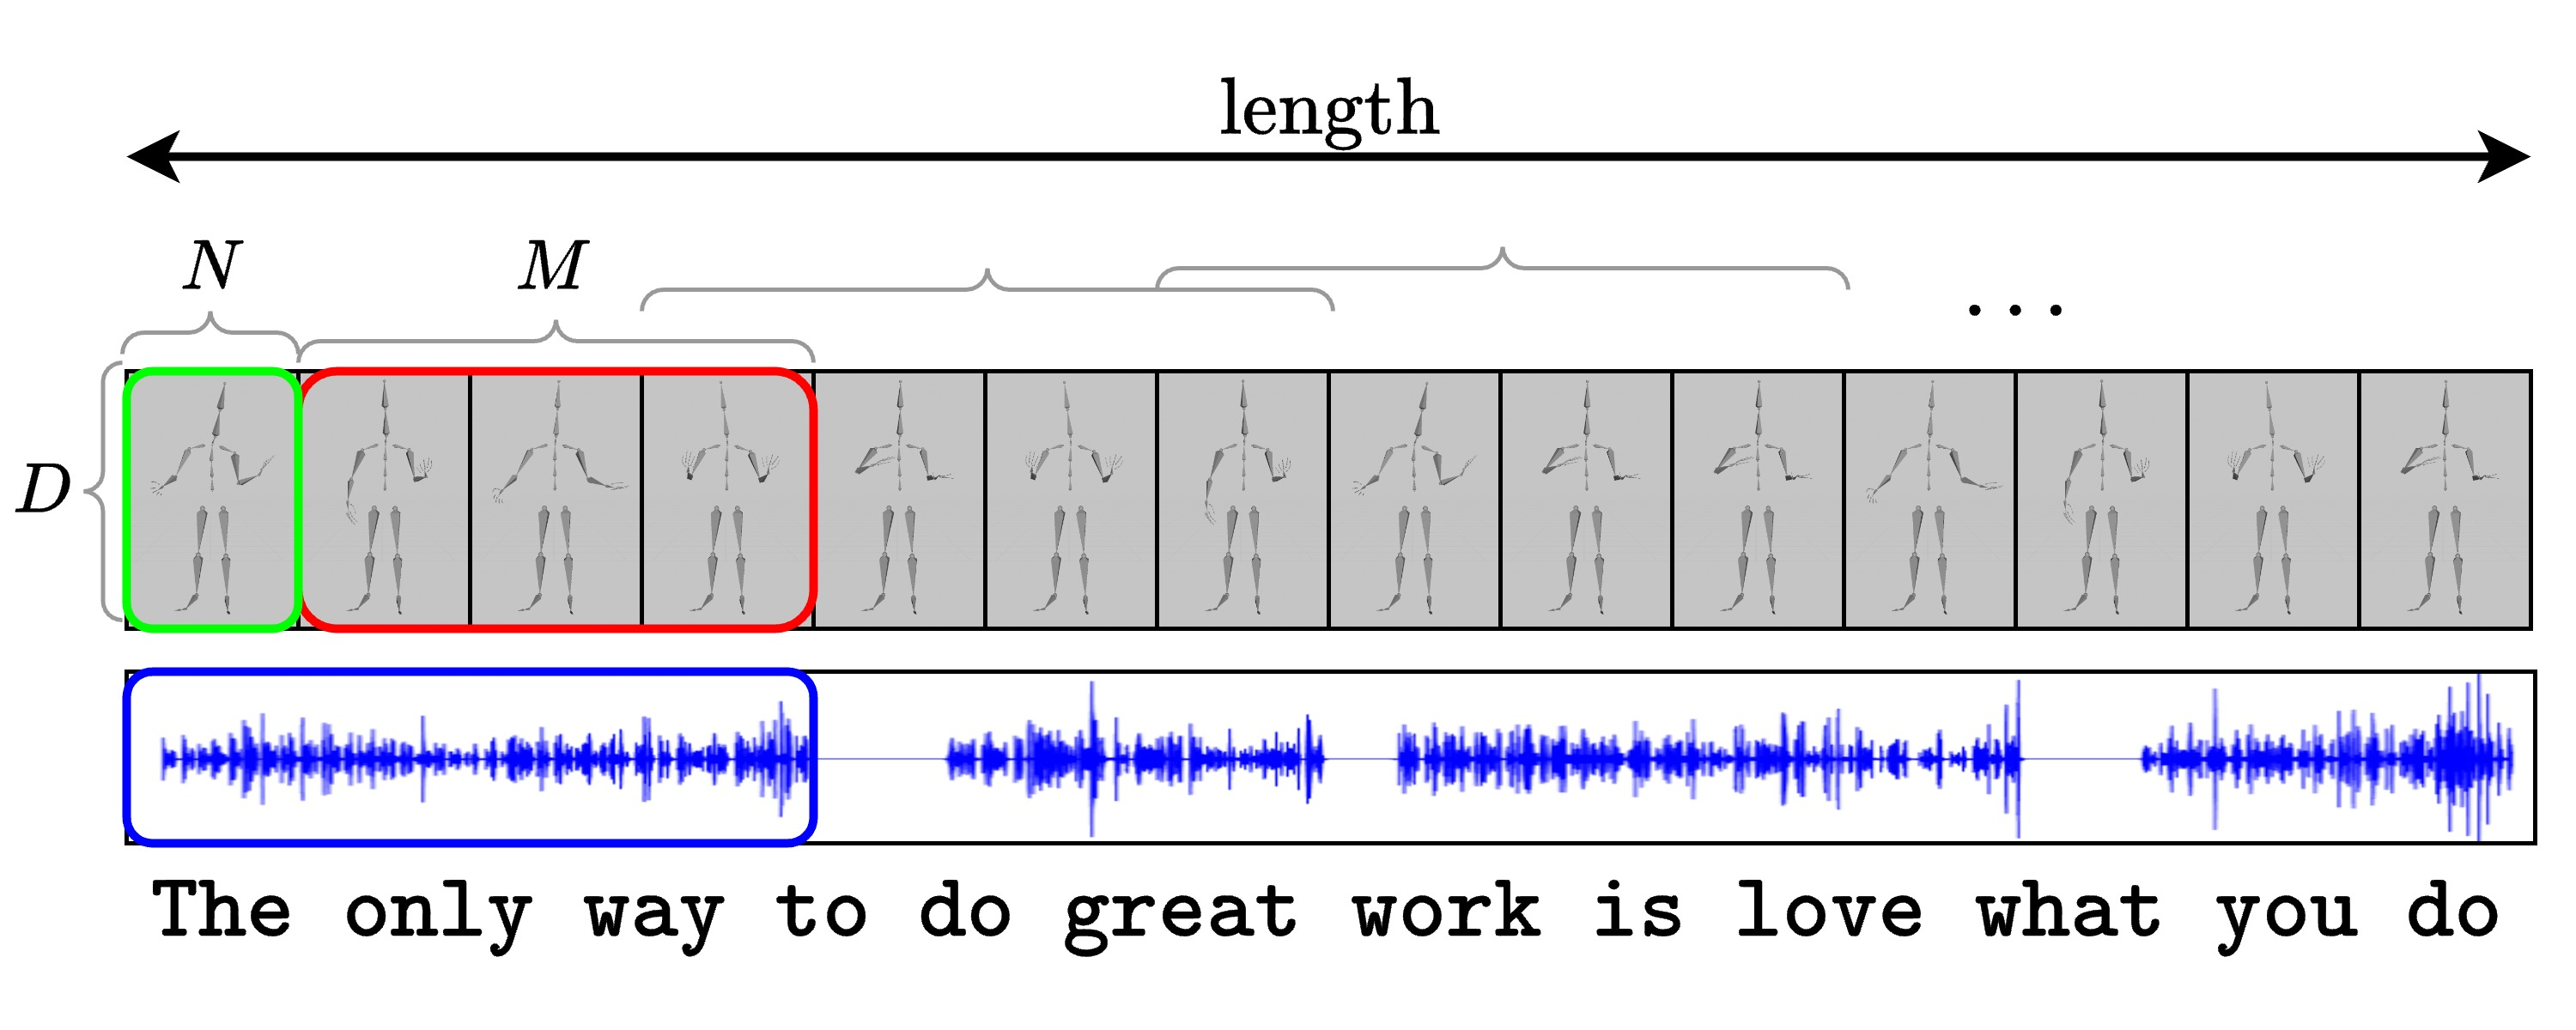
\includegraphics[height=4cm]{figures/FeatureProcessing}
			\caption{A gesture sequence: the first $N$ frames are used as seed gesture $\mathbf{s}$, and the remaining $M$ frames are to be predicted}
			\label{fig:GestureSeries}
	\end{subfigure}
\end{figure}

%\begin{figure}[h]
%	\centering
%	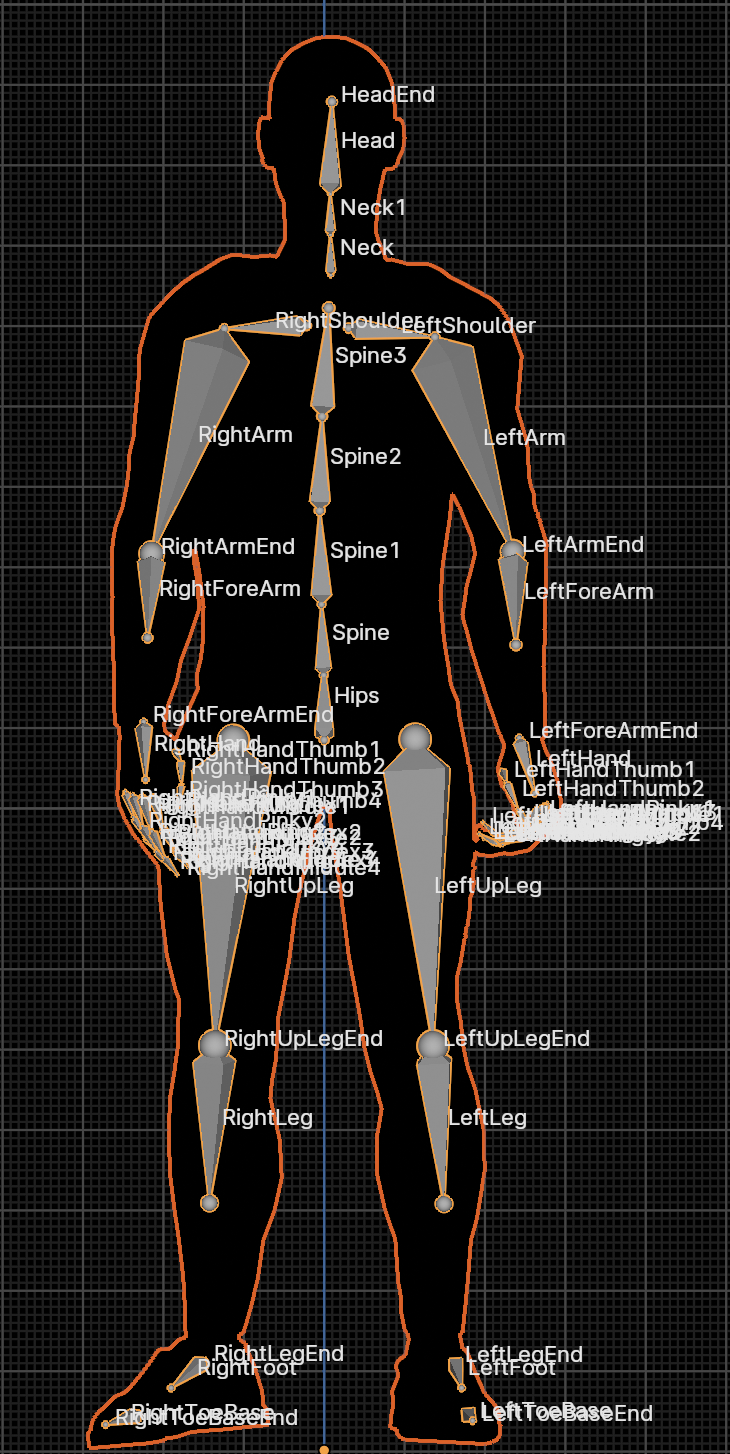
\includegraphics[height=8cm]{figures/Skeleton.png}
%	\caption{\small Skeleton and joint names of single frame}
%	\label{fig:Skeleton}
%\end{figure}

\textbf{Skeleton Structure of Gestures}: A gesture is defined as the movement of a character's entire body over time.
Each frame is a skeleton (\autoref{fig:Skeleton}) of 75 bones: $\{ \mathbf{b}_{1}, \mathbf{b}_{2}, \cdots , \mathbf{b}_{75} \}$, where each bone has position $\{ p_{x}, p_{y}, p_{z} \}$ and rotation $\{ r_{x}, r_{y}, r_{z} \}$.
%, as shown in \autoref{fig:Skeleton}, captured frame by frame. In computer graphics, character motion is represented as bone-specific movements, including hands, legs, head, spine, etc. 
%The full character skeleton structure is presented in Appendix \autoref{appendix:BVHSkeleton}.

%Motion data is captured using motion capture systems using cameras and specialized sensors. The output is typically stored in BVH (Biovision Hierarchy) files.

%A BVH file consists of two main parts: \texttt{HIERARCHY} and \texttt{MOTION}. The \texttt{HIERARCHY} section is structured as a tree containing the skeleton’s initial positions and names. The \texttt{MOTION} section contains the movement data for the entire skeleton frame-by-frame. Each BVH file includes frame rate (fps) and total frame count. Details are presented in Appendix \autoref{appendix:BVHStructure}.

\textbf{Motion Structure of Gestures}: Gesture motion data is convert from position and rotation into quaternion space to get raw motion waves. Then we apply DFT to extract cofficient \citep{suwajanakorn2017synthesizing} to get feature vector of single frame $g^{(1)} \in \mathbb{R}^{D}$ with $D = 1141$. With arbitrary length, we get matrix $\bx \in \mathbb{R}^{\text{length} \times D}$. The ultimate goal is to produce a sequence of gestures that reflect the motion of the skeleton frame by frame. This can be approached via classification, clustering, or regression. Gesture generation is approached in this work as a regression-based prediction problem, wherein the next sequence ($\mathbf{x} \in \mathbf{x}^{1:M}$) is generated conditioned on the current gesture input.

Each gesture sequence is labeled with an emotion. A key novelty of our approach is pairing the gesture sequence with both the original speech and the corresponding text (transcribed from the speech).

The objective is to build a model that predicts $M$ future frames from the given inputs: seed gesture $\mathbf{s} \in \mathbb{R}^{1:N \times D}$, speech $\mathbf{a}$, text $\mathbf{v}$, and emotion $\mathbf{e}$. The model prediction is $\hat{\mathbf{x}} \in \mathbb{R}^{1:M \times D}$, which is compared against ground-truth gesture $\mathbf{x} \in \mathbb{R}^{1:M \times D}$.

% as illustrated in \autoref{fig:Skeleton}, or the \texttt{MOTION} section of a BVH file, contains position and rotation information per frame. 

%The output of gesture generation is a sequence of bone rotations per frame. The generated gestures are evaluated based on naturalness, human-likeness, and contextual appropriateness.


%The preprocessing pipeline is detailed in \autoref{appendix:BVHData}.

%\textbf{Problem Statement}
%\label{sec:ProblemStatement}



\subsection{Challenges}
\label{sec:difficult}

There are several challenges in building a model that can learn human-like conversational gesture patterns: \textit{Scarce, Low-Quality Data}: High-quality motion capture datasets are expensive and limited.
\textit{Modal Inconsistency}: Text data outpaces speech; speaker attribution and speech-emotion synchronization are often absent, with texts covering diverse, unrelated topics.
\textit{Imbalanced Features}: Datasets favor English-speaking gestures, with uneven distributions across speaking, questioning, and silent states.
\textit{High Computational Cost}: Encoding multimodal inputs (text, speech, 3D poses) increases training and inference demands; reducing inputs degrades performance.
\textit{Sequential Processing Latency}: Sequential text and speech processing for gesture generation, combined with rendering, introduces critical latency in real-time applications.

%\begin{enumerate}
%	\item \textit{Limited and low-quality data:} Creating large-scale, high-quality datasets for motion capture is extremely costly in the industry.
%	
%	\item \textit{Inconsistent context between modalities:} Text datasets are more abundant than speech, and speaker attribution is often missing. Synchronization between speech and emotional tone is also lacking. Additionally, training texts span many unrelated topics.
%	
%	\item \textit{Imbalanced feature distributions:} Current datasets are biased toward English-speaking gestures, with imbalanced gesture distributions between speaking, questioning, and silent states.
%	
%	\item \textit{High computational cost due to multimodal input:} The model must encode text, speech, and 3D pose data, increasing the computational load during both training and inference. Reducing input information also degrades performance.
%	
%	\item \textit{Sequential preprocessing steps:} Although human-computer interaction is most effective through speech and keyboard input, processing the text and speech input for gesture generation must be done sequentially. In real-world applications, inference latency is critical, and users cannot wait long. Rendering the gestures on screen must also be optimized for speed.
%\end{enumerate}

\textbf{Contributions}: This work advances gesture generation by enhancing existing datasets through transcribing speech into text, which is incorporated as semantic features during training, and extending the conditional denoising process to include these text features. Additionally, we leverage Unity for rendering, data extraction, and visualization of gesture generation outcomes, while designing and implementing a novel rendering pipeline demonstrated within the Unity environment.

%\begin{itemize}
%	\item From existing datasets, speech is transcribed into text and used as additional semantic features for training. We extend the conditional denoising process to include text features.
%	
%%	\item Based on the DiffuseStyleGesture model, 
%	
%	\item In this work, we use Unity for rendering, data extraction, and visualization of gesture generation results.
%	
%	\item A rendering pipeline is designed and implemented in this paper, with the system demonstrated using Unity.
%\end{itemize}
%
